
\subsubsection*{Program v Prologu}
    \mdef{Program} (v Prologu) je Hornova formule obsahující pouze \myblue{programové}
    \smallskip
    
    \myblue{klauzule}, tj. \myblue{fakta} nebo \myblue{pravidla}.
    \bigskip
    
    \centerline{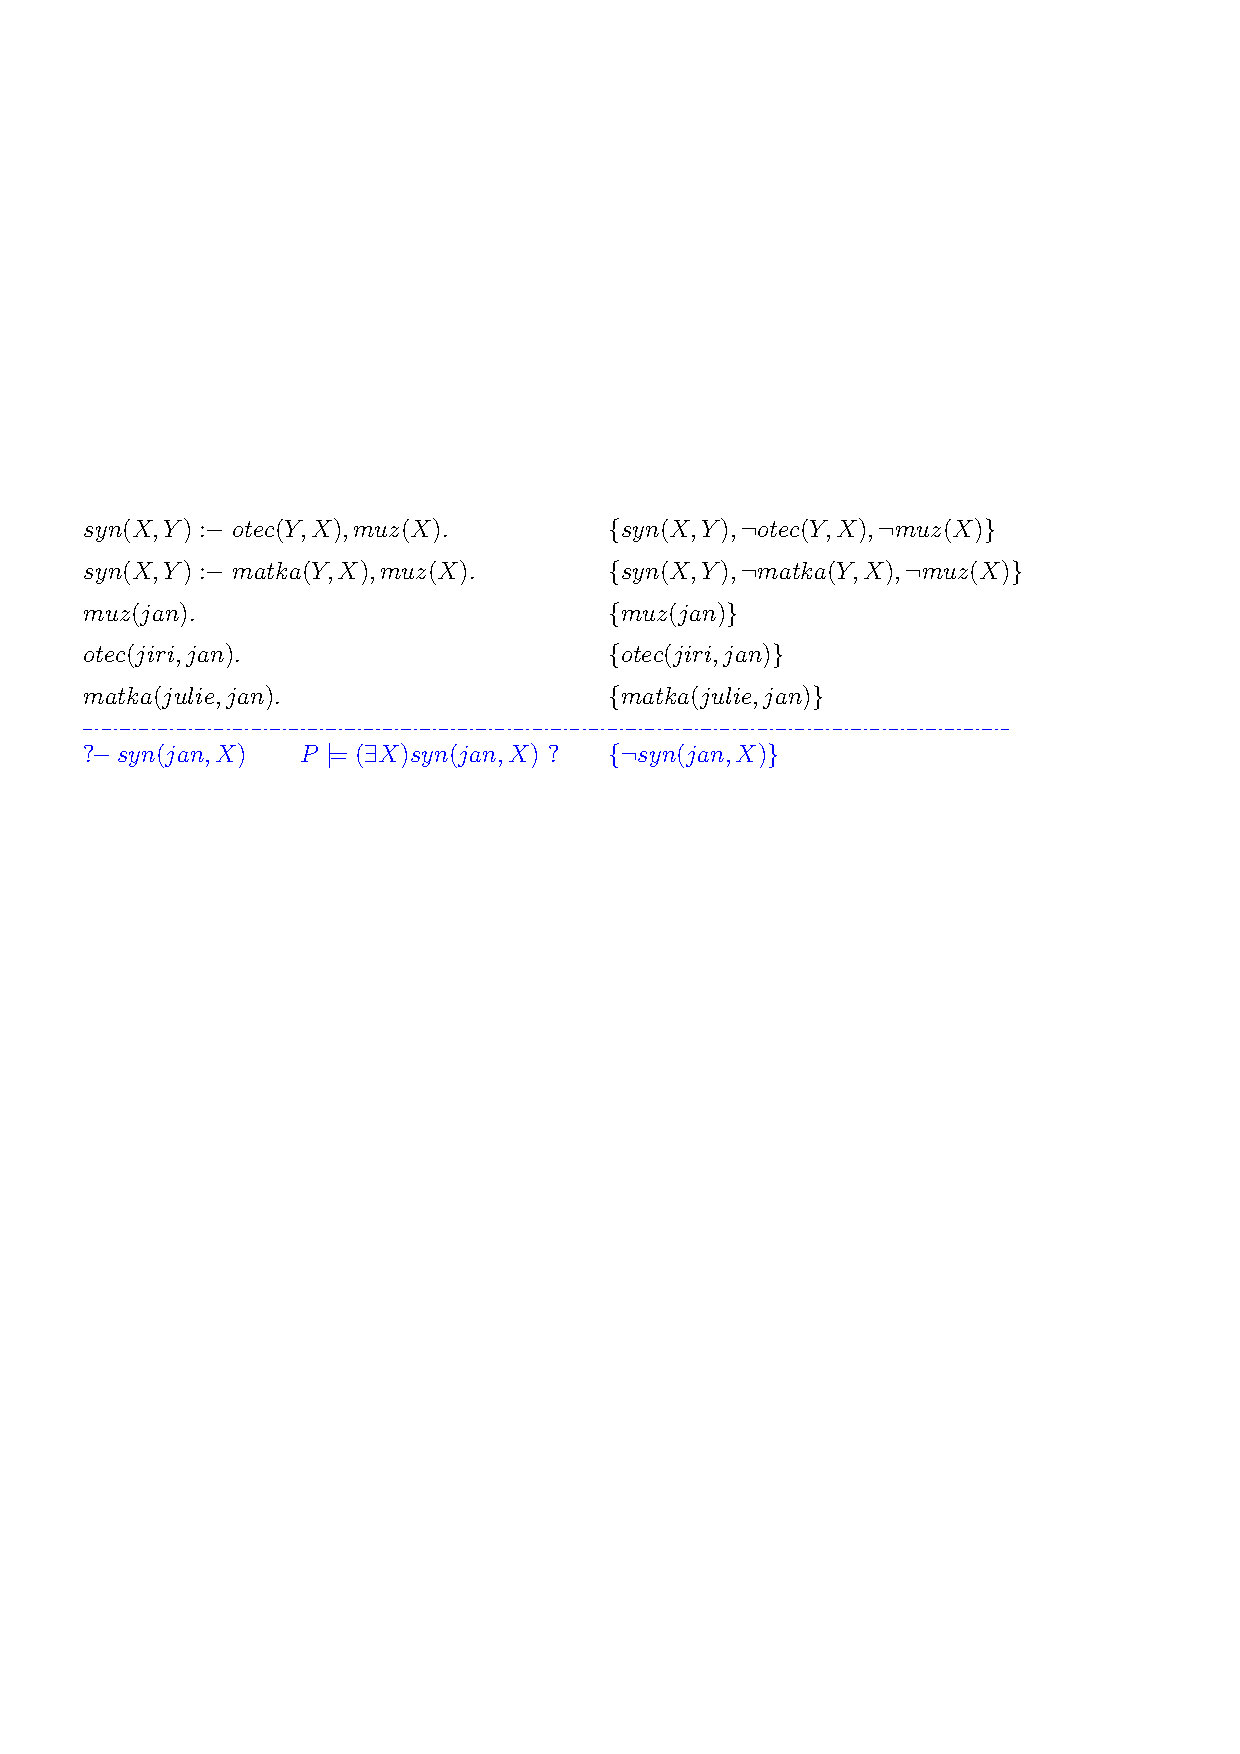
\includegraphics[scale=0.7]{files/rezolucePLprogram}}
    \bigskip
    
    {\it Zajímá nás, zda daný \myblue{existenční dotaz} vyplývá z daného programu.}%, navíc to chceme doložit \myblue{výstupní substitucí}.
    \medskip
    
    {\bf \myblue{Důsledek}}\ \ {\it Pro program $P$ a cíl $G=\{\neg A_1, \dots, \neg A_n\}$ v proměnných $X_1,\dots,X_m$
    
    \vspace{-0mm}
    \begin{enumerate}
    \item[$(1)$] $P \models (\exists X_1)\dots(\exists X_m)(A_1\mand \dots \mand A_n)$, právě když
    \smallskip
    
    \item[$(2)$] $\square$ lze odvodit LI-rezolucí z $P\cup\{G\}$ začínající (variantou) cíle $G$.
    \end{enumerate}}
    
    
    %%%%%%%%%%%%%%%%%%%%%%%%%%%%%%%%%%%%%%%%%%%%%%%%%%%%%%5
    
    \subsubsection*{LI-rezoluce nad programem}
    {\it Je-li odpověď na dotaz kladná, chceme navíc znát výstupní substituci.}
    \medskip
    
    \mdef{Výstupní substituce} $\sigma$ LI-rezoluce $\square$ z $P\cup\{G\}$ začínající $G=\{\neg A_1,\dots,\neg A_n\}$
    \smallskip
    
    je složení \myblue{mgu} v jednotlivých krocích (jen na proměnné v $G$). Platí,
    \vspace{-2mm}
    \mygreen{$$P \models (A_1 \mand \dots \mand A_n)\sigma.$$}
    
    \vspace{-2mm}
    
    \centerline{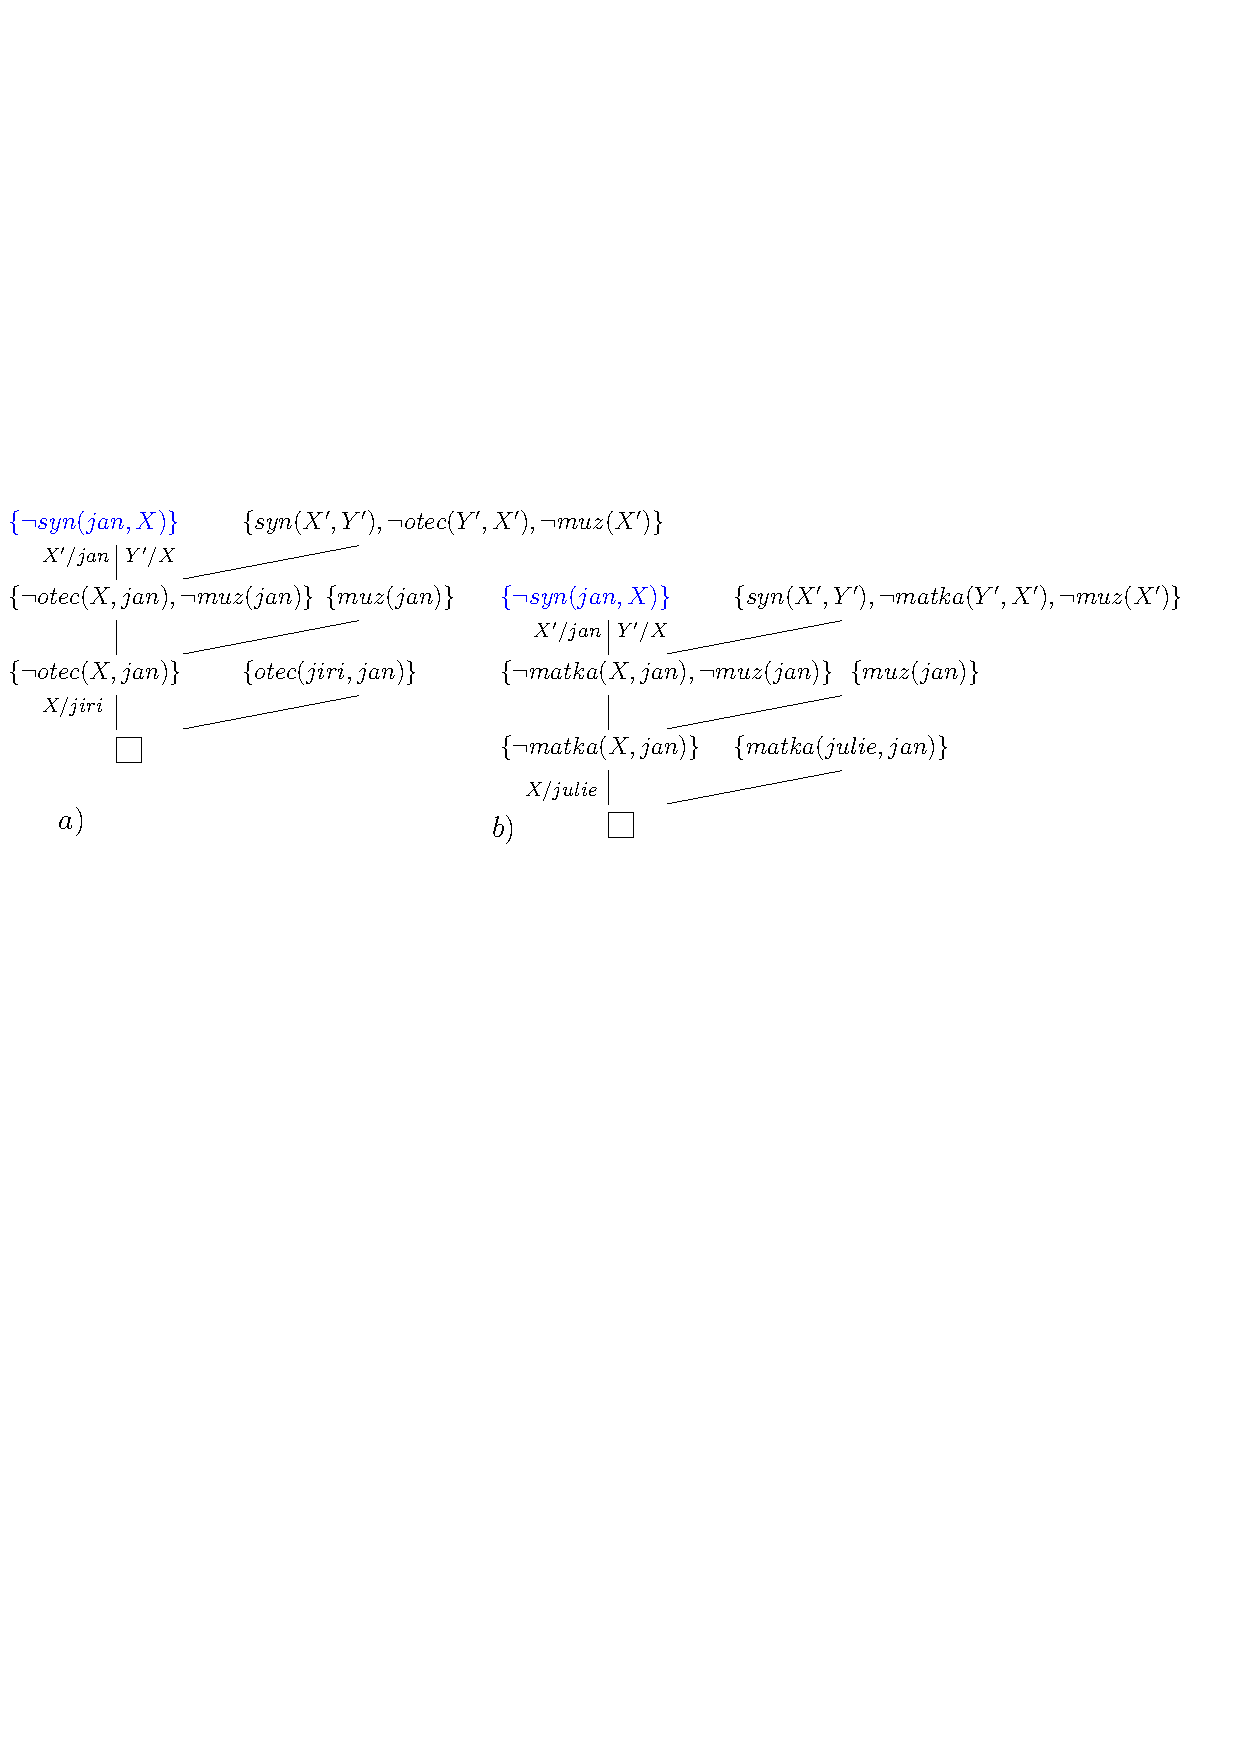
\includegraphics[scale=0.63]{files/rezolucePLprogramLI}}
    \bigskip
    
    Výstupní substituce $a)$ $X=jiri$,\ \ $b)$ $X=julie$.
    
